% ═══════════════════════════════════════════════════════════════════
% CHAPITRE 3 : CONCEPTION
% ═══════════════════════════════════════════════════════════════════

\chapter{Conception}

Le présent chapitre traduit les besoins spécifiés au chapitre 2 en une solution de conception : architecture logicielle et sa justification, modèle de classes, modèle de données, comportements dynamiques (diagrammes de séquence) et maquette de l'interface.

\section{Architecture logicielle}

\subsection{Choix d'une architecture trois-tiers}

La spécification des besoins a conduit à la mise en place d'une \textbf{architecture trois-tiers}, séparant la présentation, le traitement et la persistance (figure~\ref{fig:architecture}).

\begin{figure}[H]
\centering
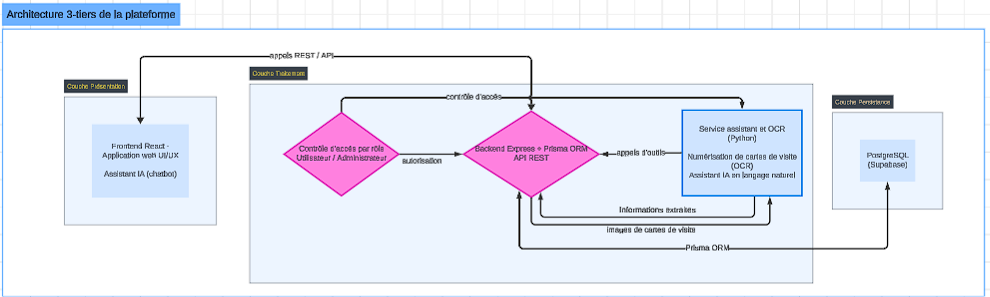
\includegraphics[width=1\textwidth]{images/architecture.png}
\caption{Architecture logicielle trois-tiers de la plateforme}
\label{fig:architecture}
\end{figure}

Ce choix répond à trois exigences posées au chapitre 2, détaillées dans le tableau~\ref{tab:exigences-archi}.

\begin{table}[H]
\centering
\small
\begin{tabularx}{\textwidth}{|l|X|}
\hline
\textbf{Plan} & \textbf{Justification} \\
\hline
Sécurité & Séparer le frontend du backend permet de n'exposer que des \acf{API} contrôlées et de protéger les accès à la base de données, jamais accessible directement par le client \\
\hline
Maintenabilité & La séparation des couches permet de faire évoluer chaque partie indépendamment sans impact sur les autres \\
\hline
Déploiement & Chaque couche peut être hébergée et dimensionnée sur une infrastructure adaptée \\
\hline
\end{tabularx}
\caption{Justification de l'architecture trois-tiers}
\label{tab:exigences-archi}
\end{table}

\subsection{Répartition des composants}

L'architecture distingue trois composants principaux, dont les rôles sont rassemblés dans le tableau~\ref{tab:composants}.

\begin{table}[H]
\centering
\small
\begin{tabularx}{\textwidth}{|l|X|}
\hline
\textbf{Composant} & \textbf{Rôle} \\
\hline
Frontend & Application web \acf{UI}/\acf{UX} chargée de l'affichage et de l'interaction : couche de présentation communiquant avec le backend par des appels \acf{REST}, et hébergeant le widget de l'assistant \\
\hline
Backend & Expose les \acf{API} \acf{REST} et porte la logique métier : gestion des contacts, de l'authentification et du contrôle d'accès, de l'import et de l'export. Il assure la persistance des données \\
\hline
Service assistant \& OCR & Service Python dédié portant d'une part la numérisation de cartes de visite (traitement d'images) et d'autre part l'assistant IA répondant en langage naturel, qui interroge le backend par appels d'outils \\
\hline
\end{tabularx}
\caption{Répartition des composants de l'architecture}
\label{tab:composants}
\end{table}

Le recours à un \textbf{service Python dédié} pour la numérisation OCR repose sur un écosystème de bibliothèques mature en Python (reconnaissance optique, prétraitement d'images, détection de zones textuelles). Ce même service héberge également l'\textbf{assistant IA} en langage naturel, qui sollicite le backend par des appels d'outils. Sa mise en œuvre est approfondie au chapitre de la réalisation.

\section{Modèle de classes}

Le modèle de classes de la plateforme est représenté à la figure~\ref{fig:classes}. Il traduit la structuration des entités du domaine identifiées lors de l'analyse des besoins.

\begin{figure}[H]
\centering
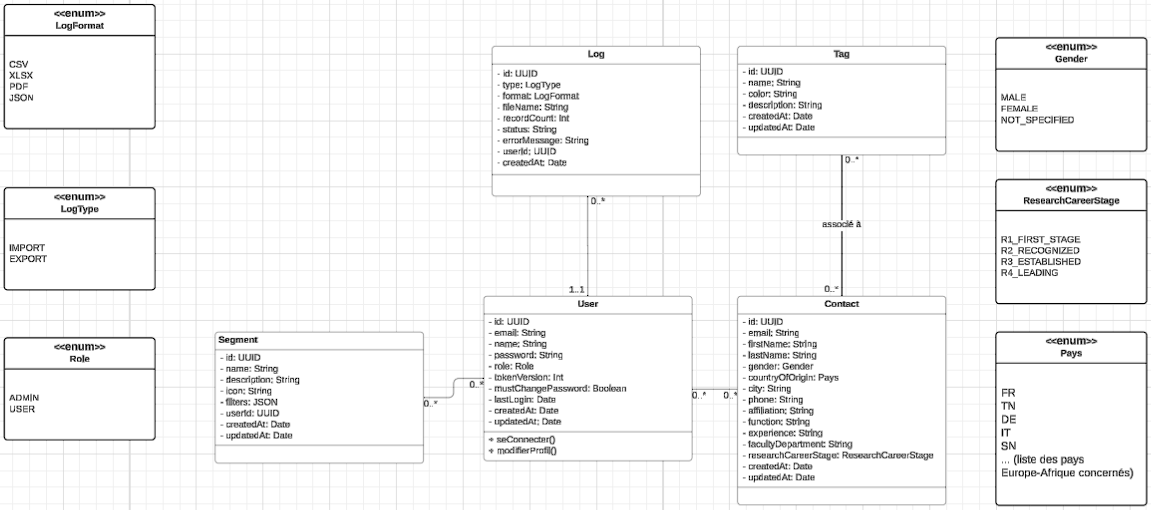
\includegraphics[width=1\textwidth]{images/diagramme_classes.png}
\caption{Diagramme de classes du système}
\label{fig:classes}
\end{figure}

La lecture de ce modèle met en évidence les relations clés du domaine, décrites dans le tableau~\ref{tab:entites}.

\begin{table}[H]
\centering
\small
\begin{tabularx}{\textwidth}{|l|X|}
\hline
\textbf{Entité} & \textbf{Rôle} \\
\hline
\texttt{User} & Modélise les comptes ; porte les attributs \texttt{role} (Utilisateur ou Administrateur) et \texttt{privilege}, support du contrôle d'accès \\
\hline
\texttt{Contact} & Représente les experts du réseau ; agrège l'ensemble des informations de la fiche (coordonnées, affiliation, fonction, stage de carrière) \\
\hline
\texttt{Tag} & Permet de catégoriser les contacts, un contact pouvant porter plusieurs tags et un tag s'appliquant à plusieurs contacts \\
\hline
\texttt{Segment} & Permet de conserver un ensemble de filtres sauvegardés afin de constituer des sous-ensembles de contacts \\
\hline
\end{tabularx}
\caption{Entités principales du domaine et leurs rôles}
\label{tab:entites}
\end{table}

Le choix de représenter le \textbf{stage de carrière} et le \textbf{genre} par des énumérations, plutôt que par des champs libres, contraint les valeurs possibles, évite les fautes de saisie et facilite le filtrage et les statistiques : une normalisation volontaire au service d'une exploitation fiable du réseau.

\section{Modèle de données}

Le modèle de données relationnel découle directement du modèle de classes et est implémenté avec l'\acf{ORM} Prisma sur une base PostgreSQL. Quelques contraintes en garantissent l'intégrité :
\begin{itemize}[leftmargin=*,itemsep=2pt]
  \item un identifiant de type UUID pour chaque entité.
  \item une adresse électronique unique pour les contacts, clé de déduplication lors des imports.
  \item la suppression en cascade des associations d'un contact ou d'un tag.
  \item des index sur les colonnes de filtres fréquents (pays d'origine du contact, associations de tags) pour accélérer la recherche et la segmentation.
\end{itemize}

\section{Diagrammes de séquence}

Pour illustrer les comportements dynamiques les plus significatifs, deux scénarios à forte valeur technique sont présentés : la consultation de la base via l'assistant IA et la numérisation d'une carte de visite.

Le premier scénario (figure~\ref{fig:seq-assistant}) illustre une consultation de la base en langage naturel. L'utilisateur pose sa question dans le widget de l'assistant. La requête est relayée au service assistant via le backend, qui la soumet au modèle de langage. Celui-ci sélectionne l'outil approprié parmi ceux exposés (recherche de contacts, synthèse d'un contact, statistiques). L'outil interroge alors le backend, dont les résultats reviennent au service, lequel formule une réponse affichée dans le widget.

\begin{figure}[H]
\centering
\includegraphics[width=0.8\textwidth]{images/sequence_assistant.png}
\caption{Diagramme de séquence : consultation de la base via l'assistant IA}
\label{fig:seq-assistant}
\end{figure}

Le deuxième scénario (figure~\ref{fig:seq-import}) déroule la numérisation d'une carte de visite. Après authentification, l'utilisateur transmet l'image au service OCR via le backend. Le service analyse l'image, en extrait les informations structurées et les renvoie au backend, qui pré-remplit la fiche de contact. Celle-ci est proposée à l'utilisateur pour validation avant enregistrement.

\begin{figure}[H]
\centering
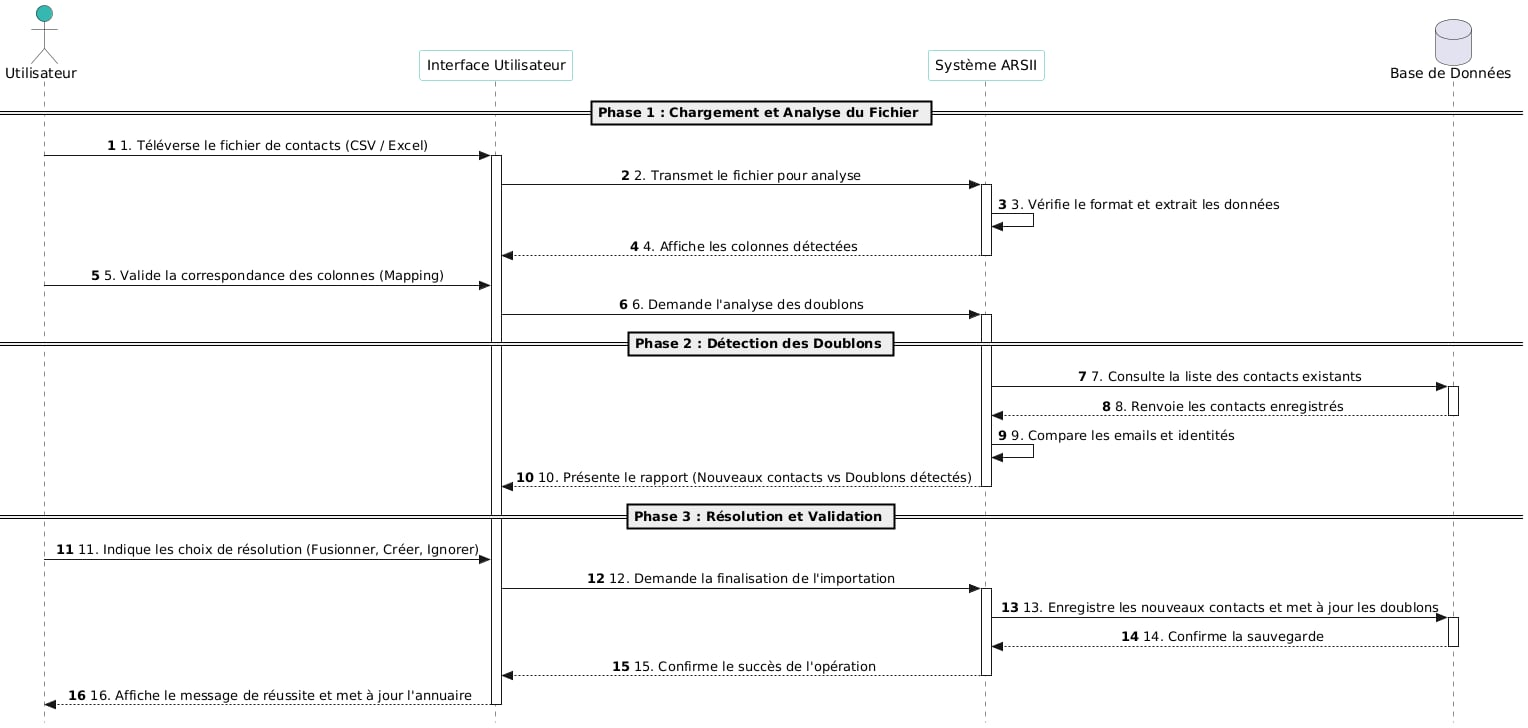
\includegraphics[width=0.8\textwidth]{images/sequence_import.png}
\caption{Diagramme de séquence : numérisation OCR d'une carte de visite}
\label{fig:seq-import}
\end{figure}

\section{Maquettage de l'interface}

La conception de l'interface a été menée à partir de maquettes établies au préalable, qui ont guidé le développement de chaque module et posent le cadre général de l'ergonomie et de la navigation.

\begin{figure}[H]
\centering
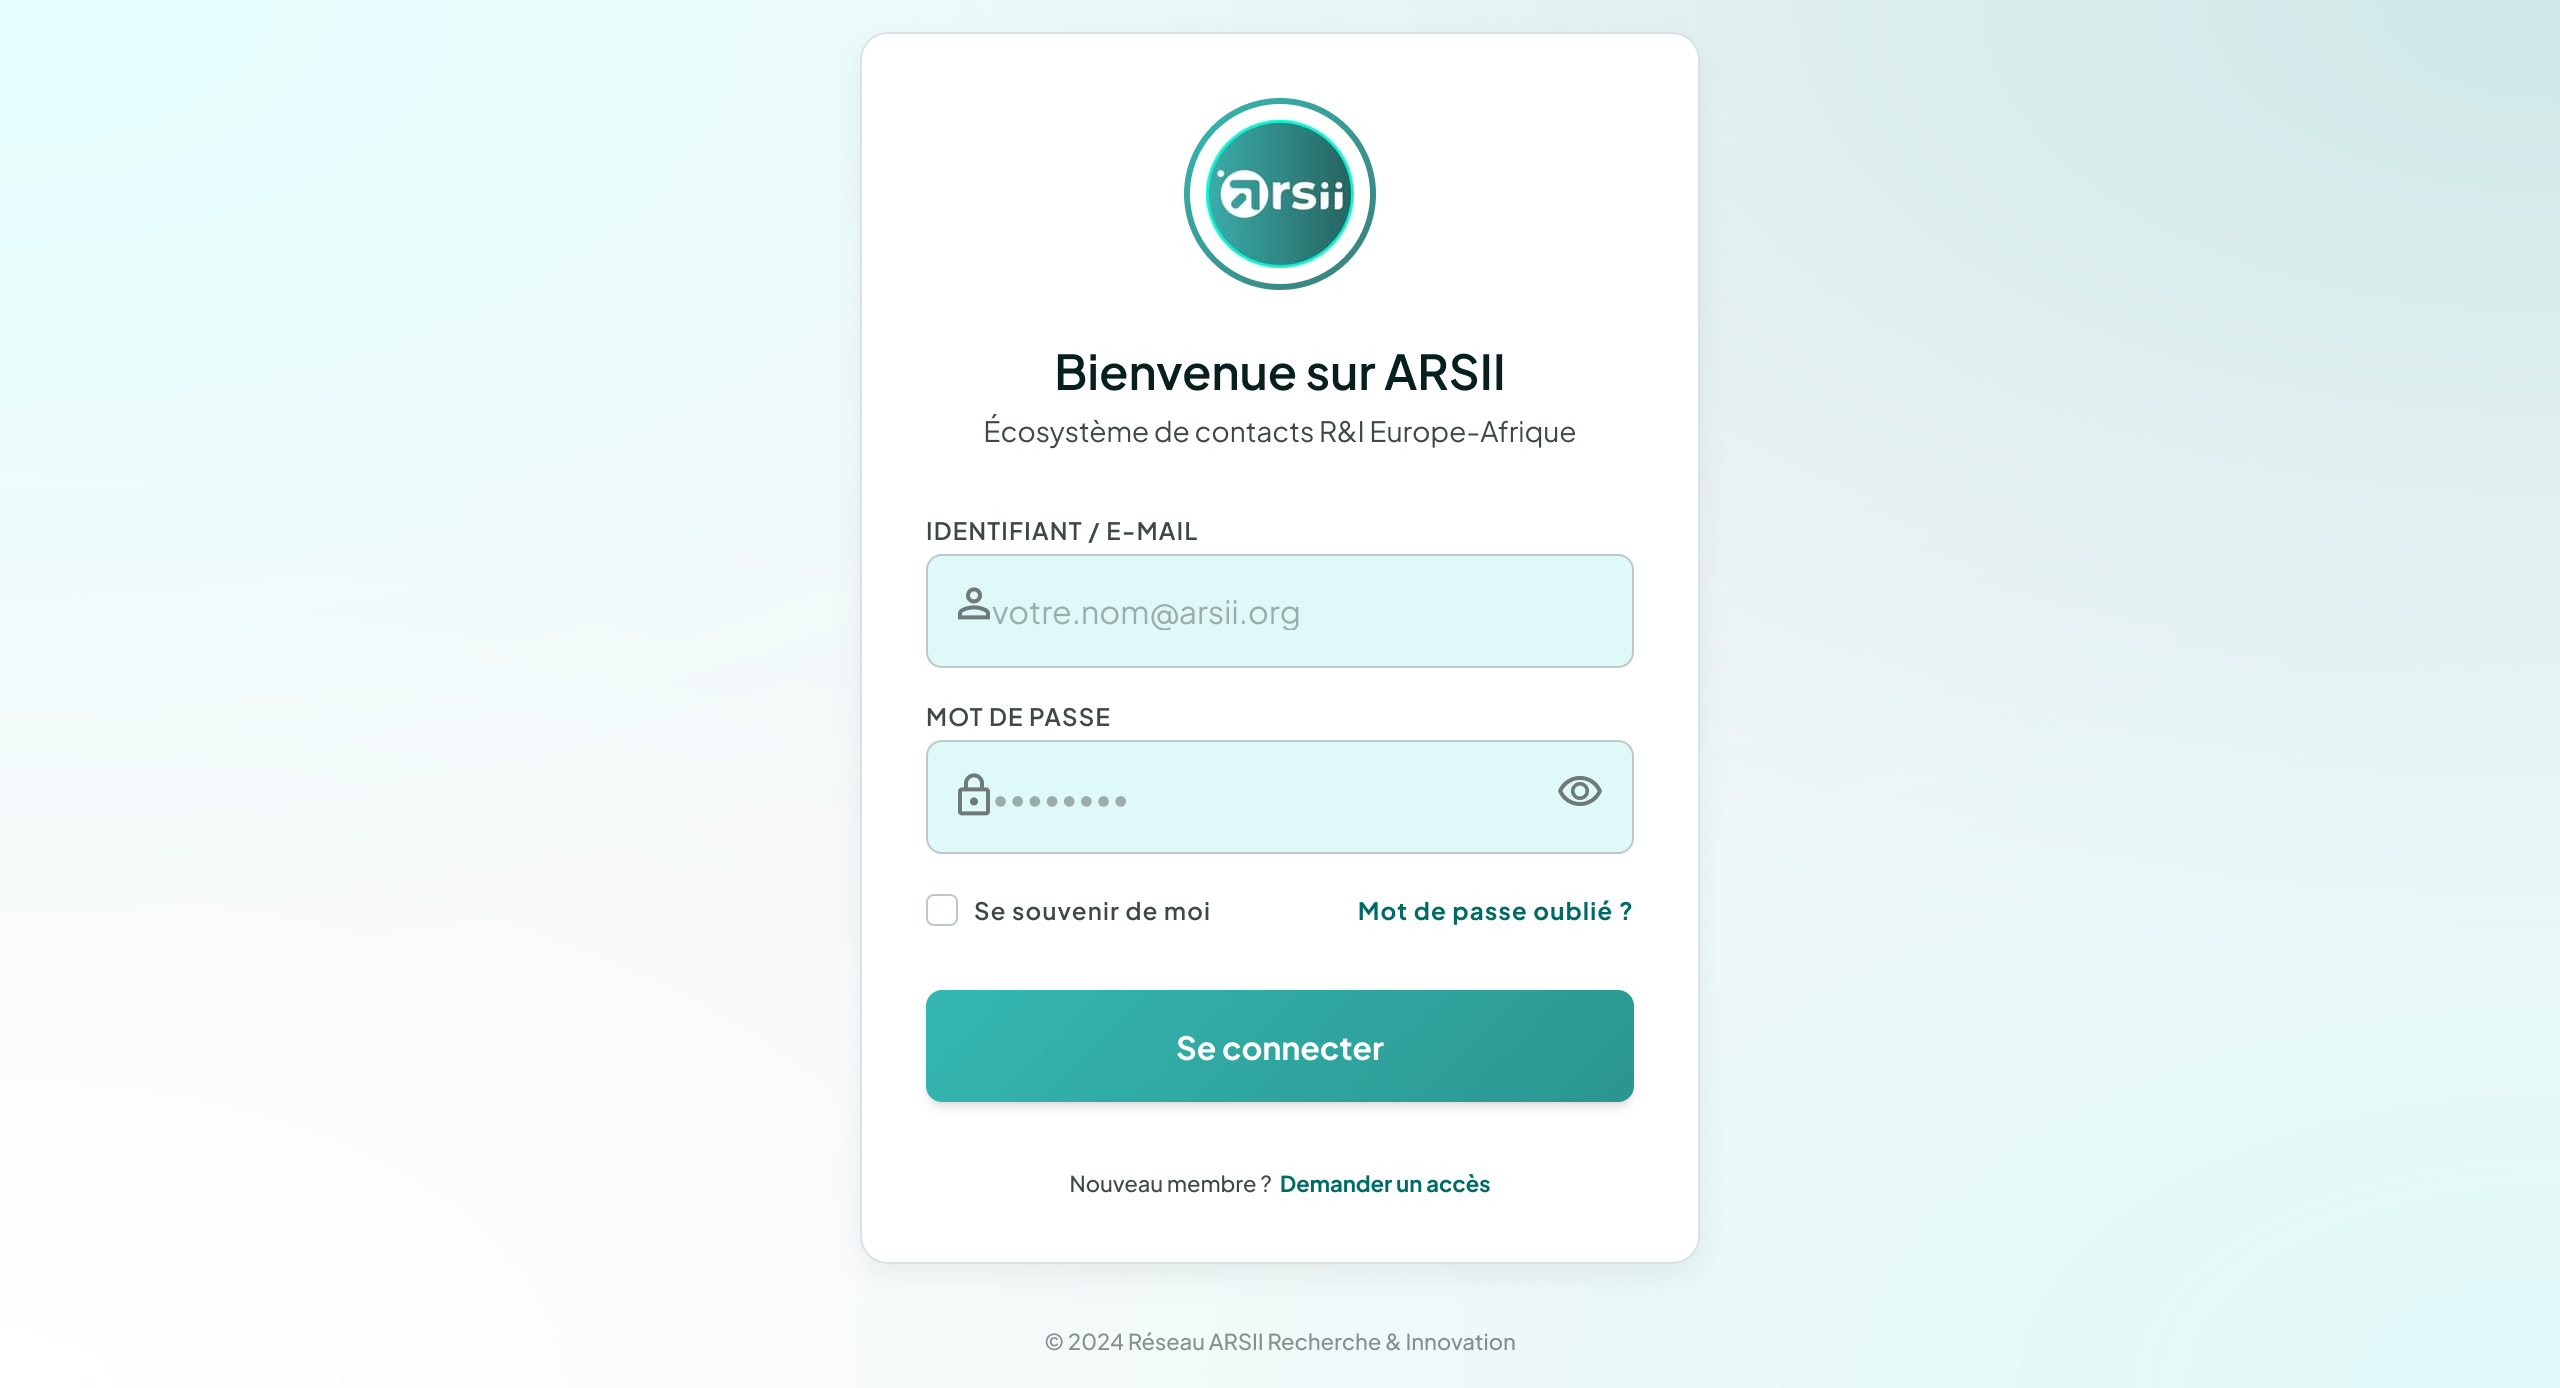
\includegraphics[width=0.8\textwidth]{images/maquette_connexion.png}
\caption{Maquette : écran de connexion}
\label{fig:maquette-connexion}
\end{figure}

\begin{figure}[H]
\centering
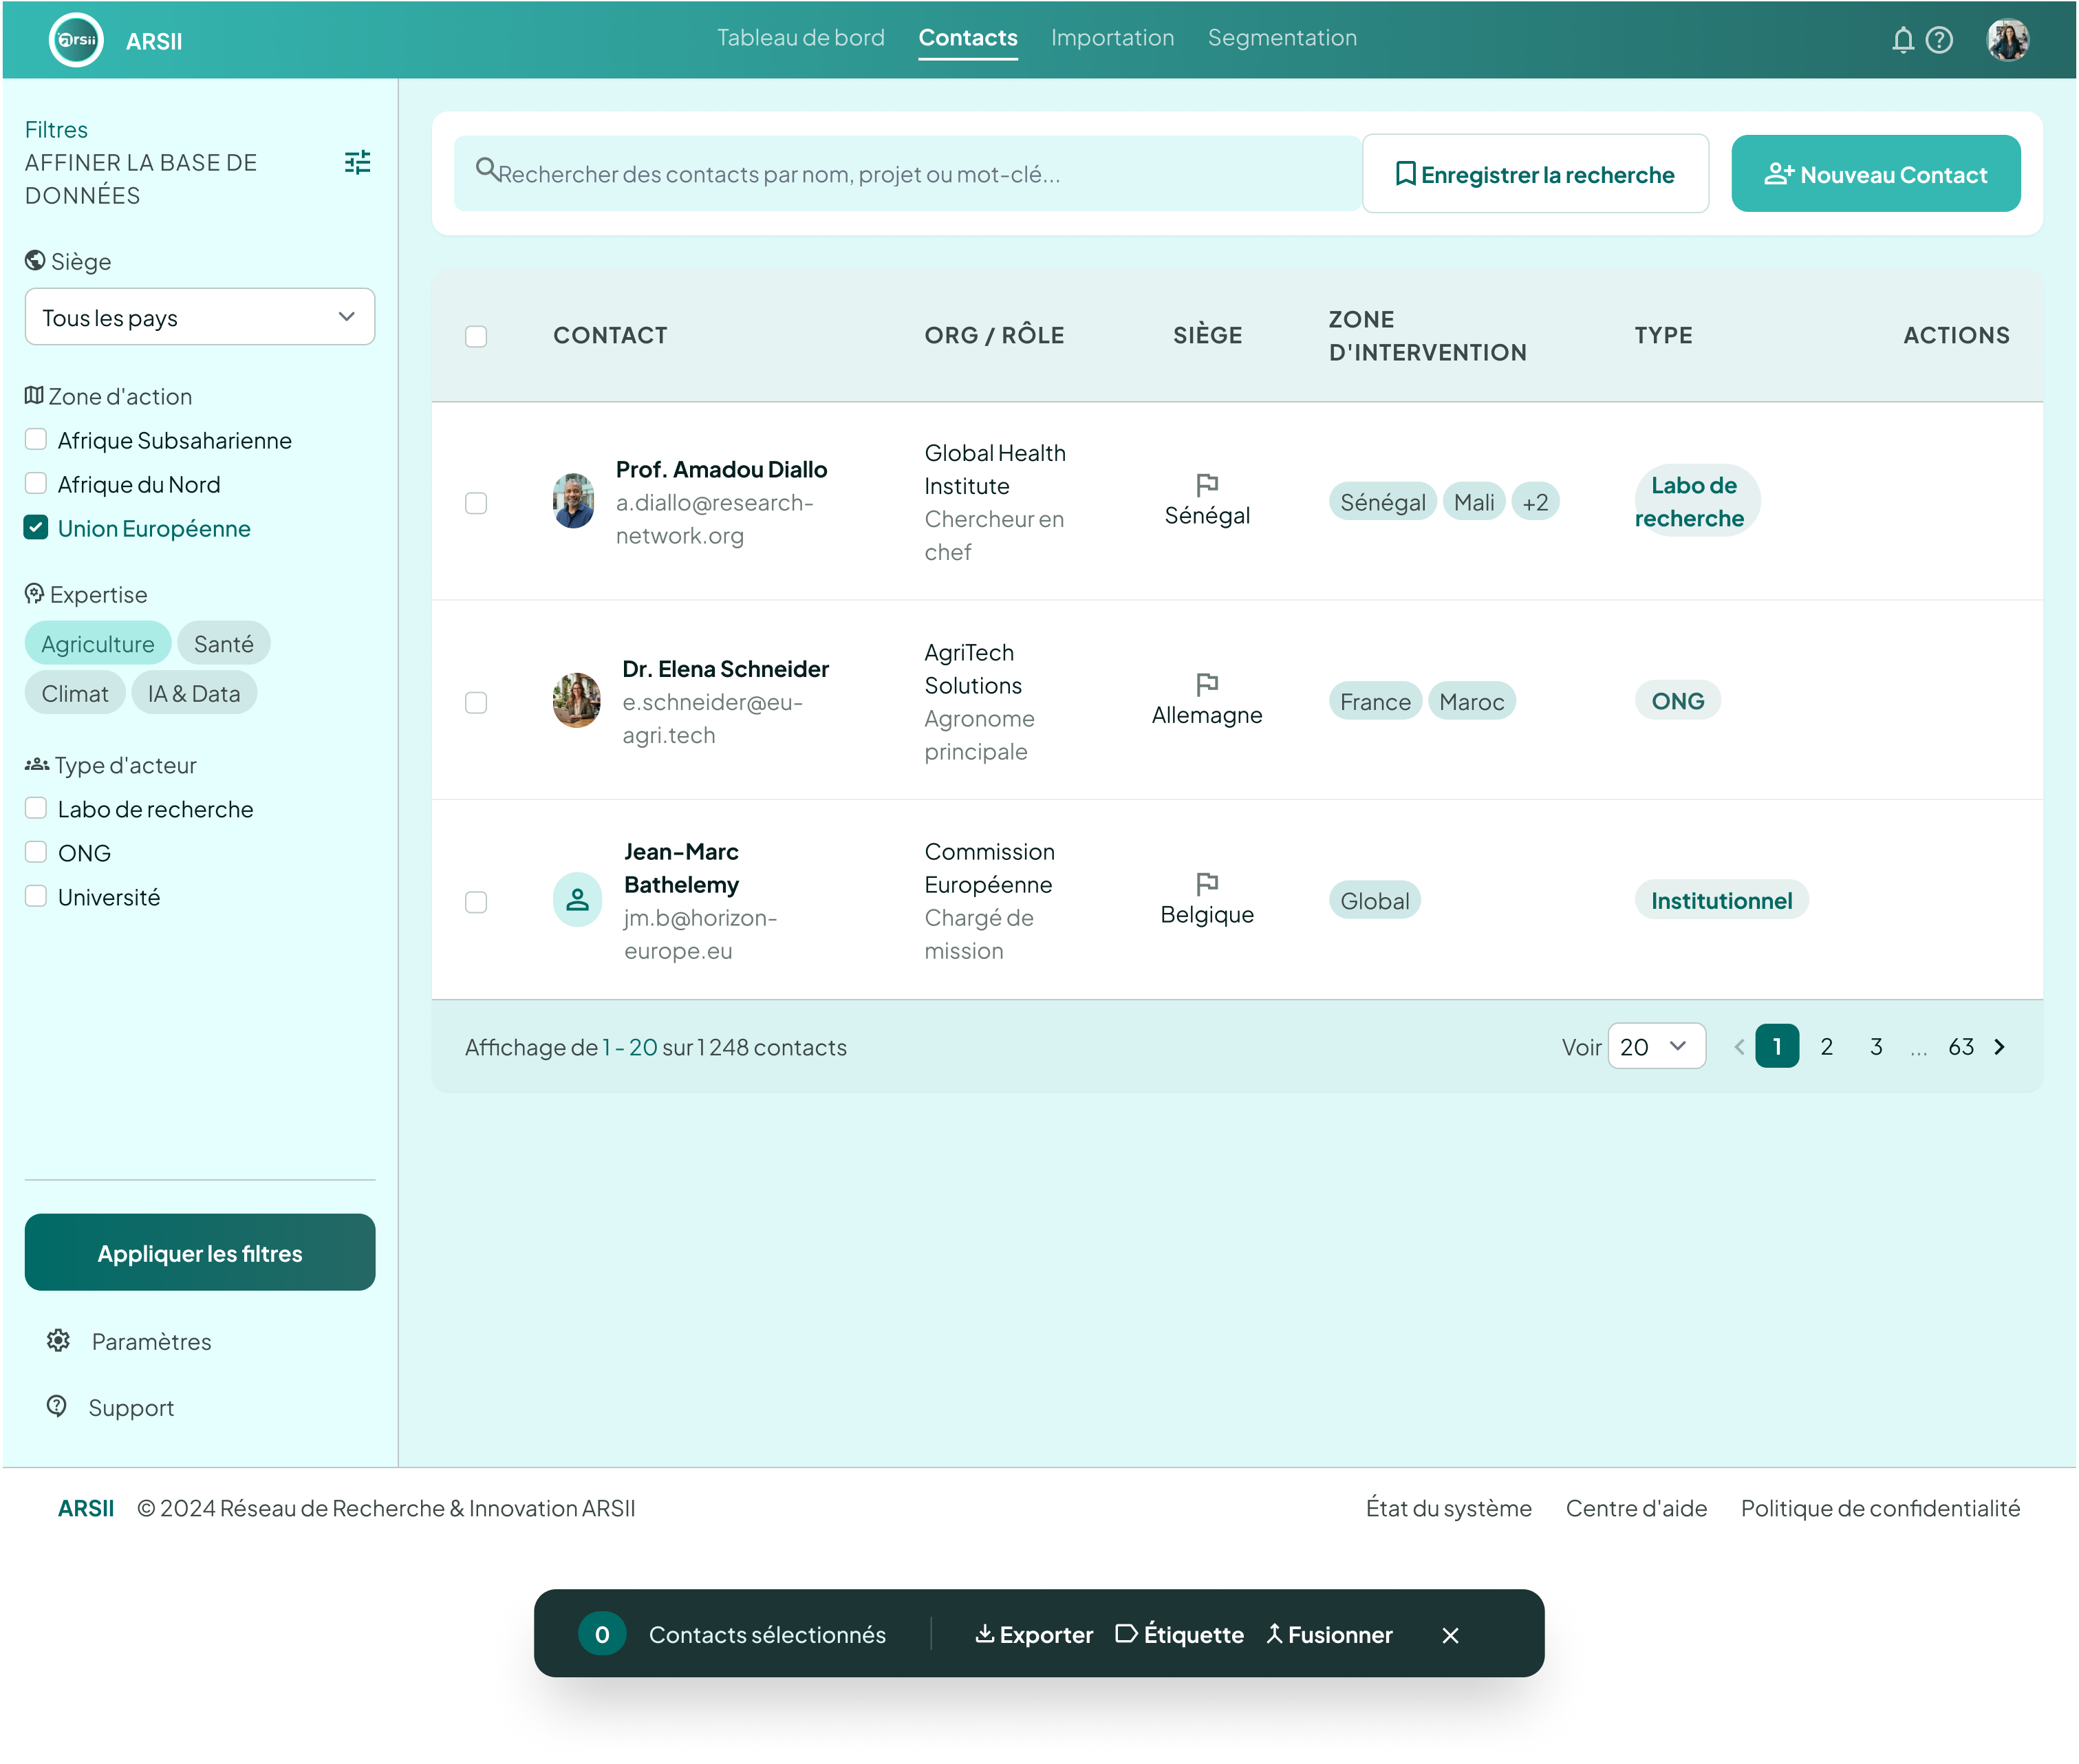
\includegraphics[width=0.9\textwidth]{images/maquette_liste_contacts.png}
\caption{Maquette : liste des contacts}
\label{fig:maquette-liste}
\end{figure}

\begin{figure}[H]
\centering
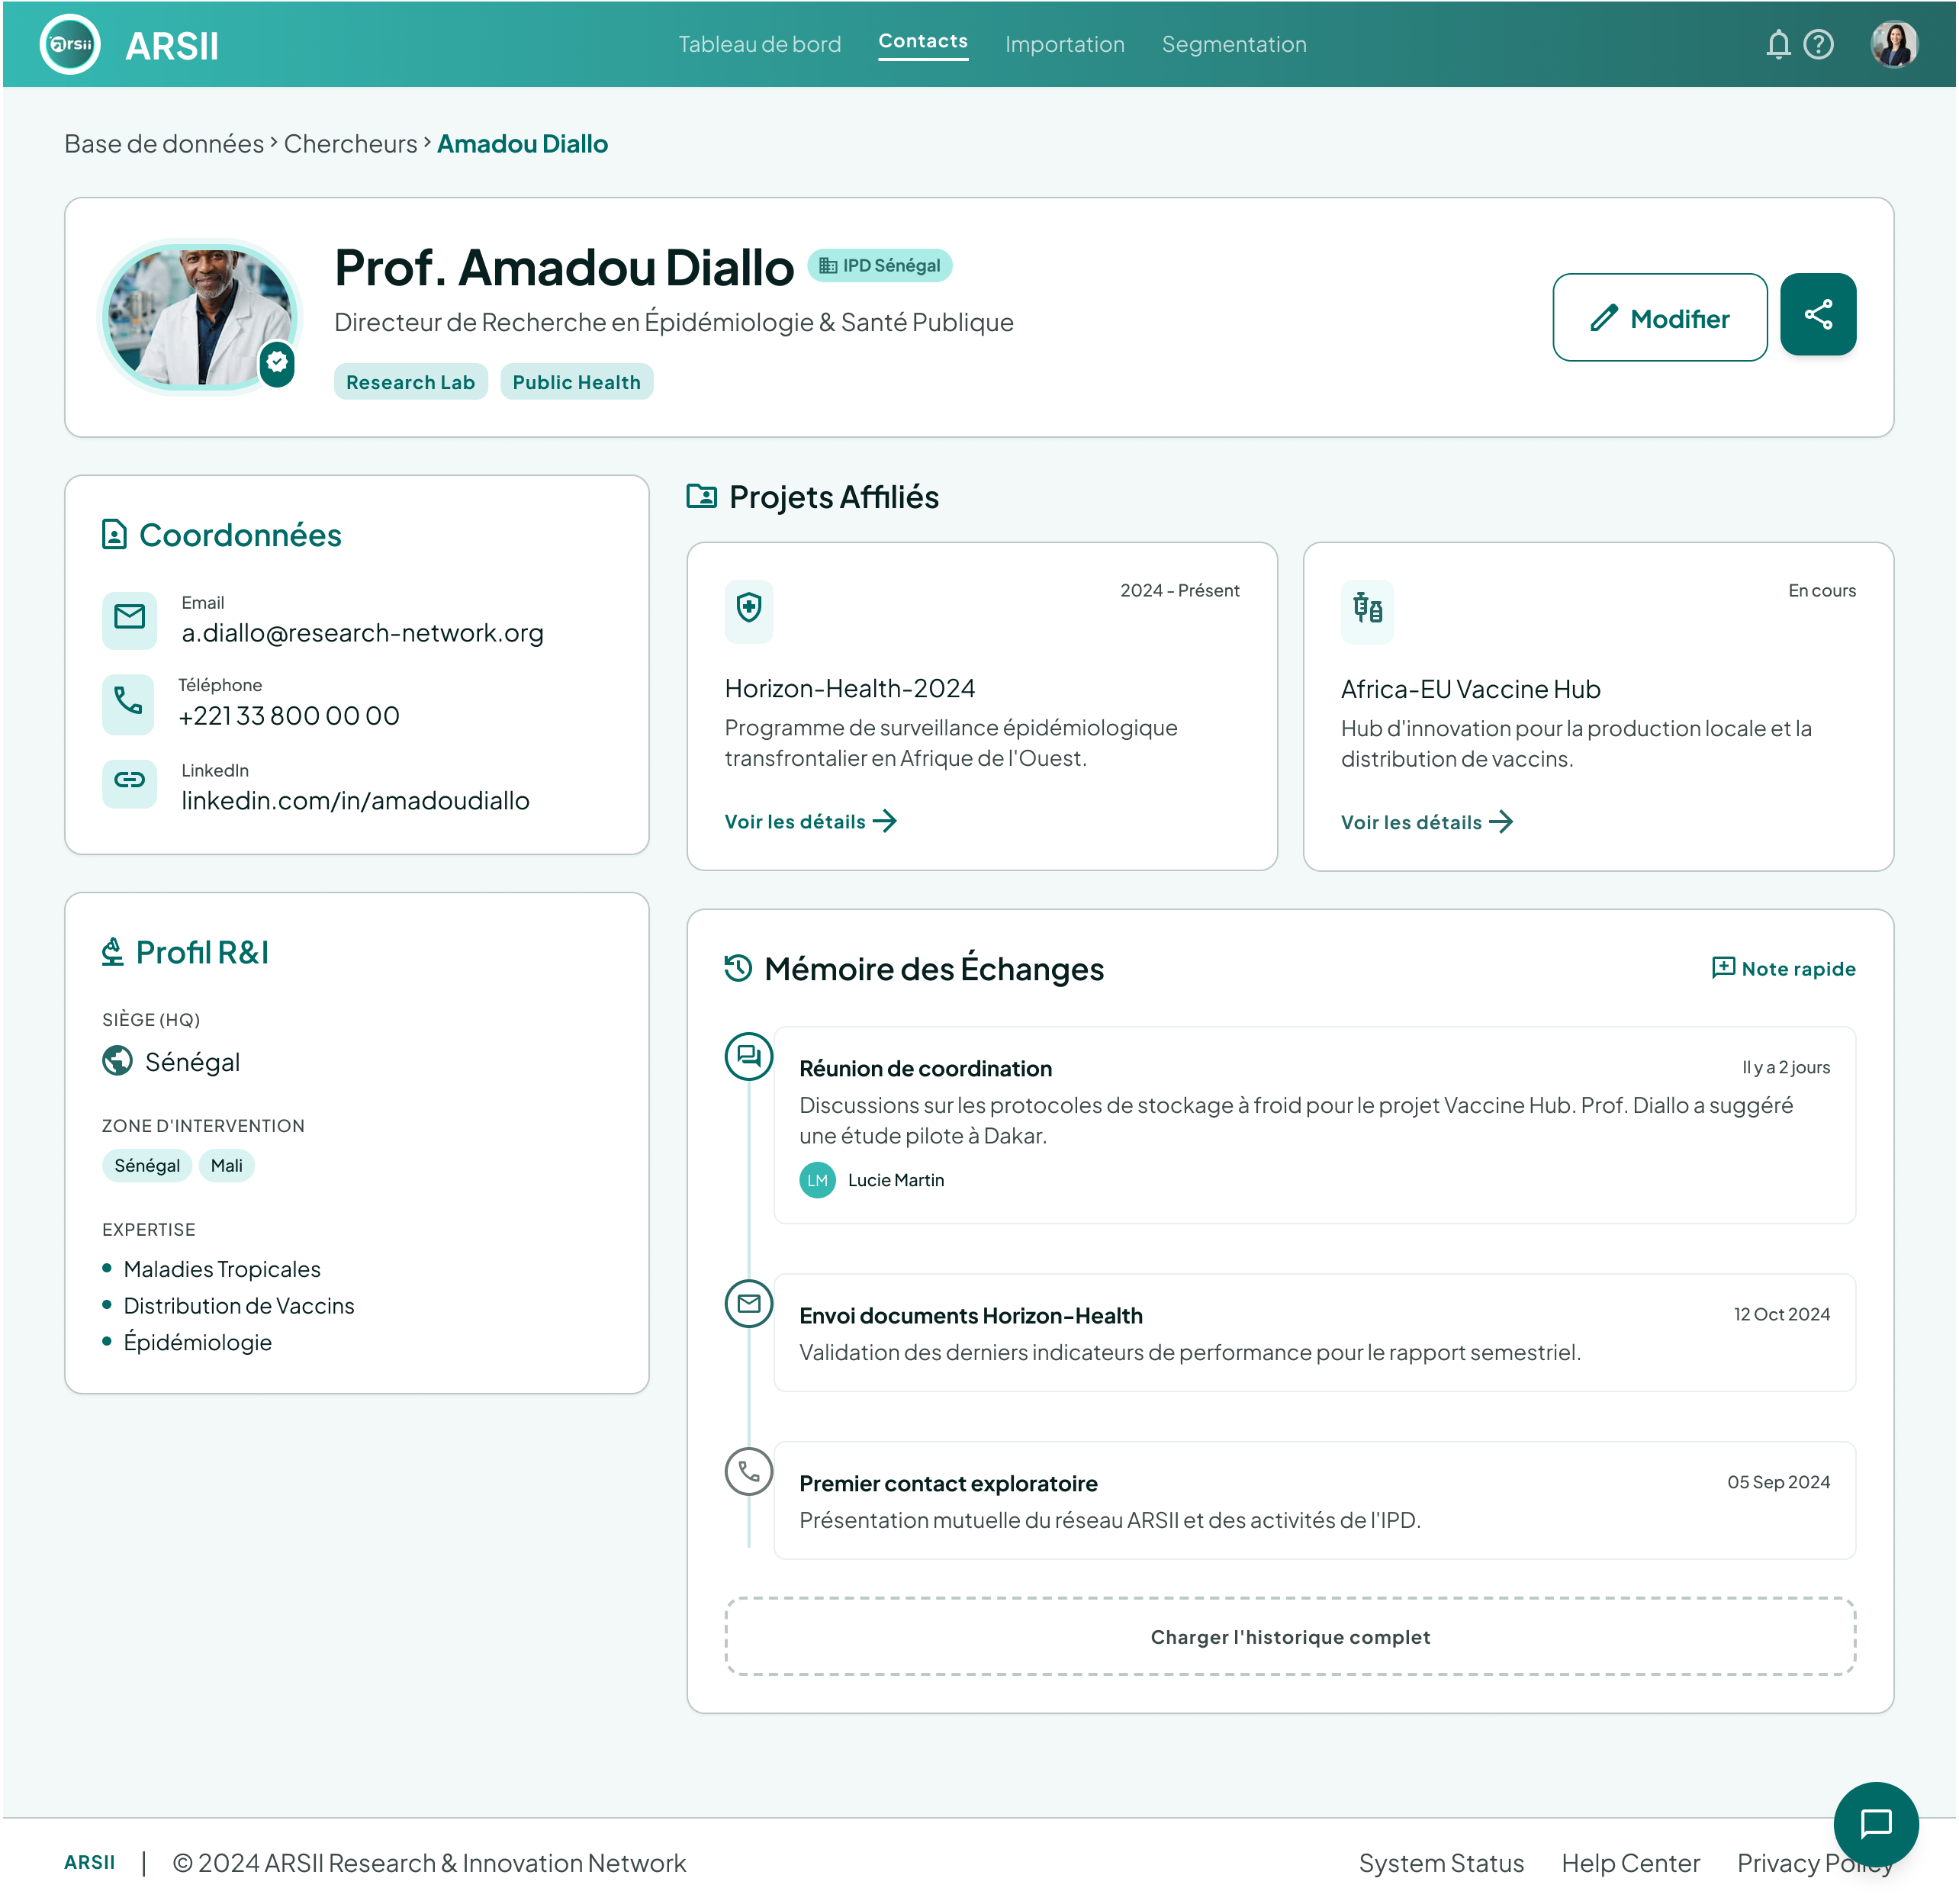
\includegraphics[width=0.9\textwidth]{images/maquette_fiche_contact.png}
\caption{Maquette : fiche contact}
\label{fig:maquette-fiche}
\end{figure}

\begin{figure}[H]
\centering
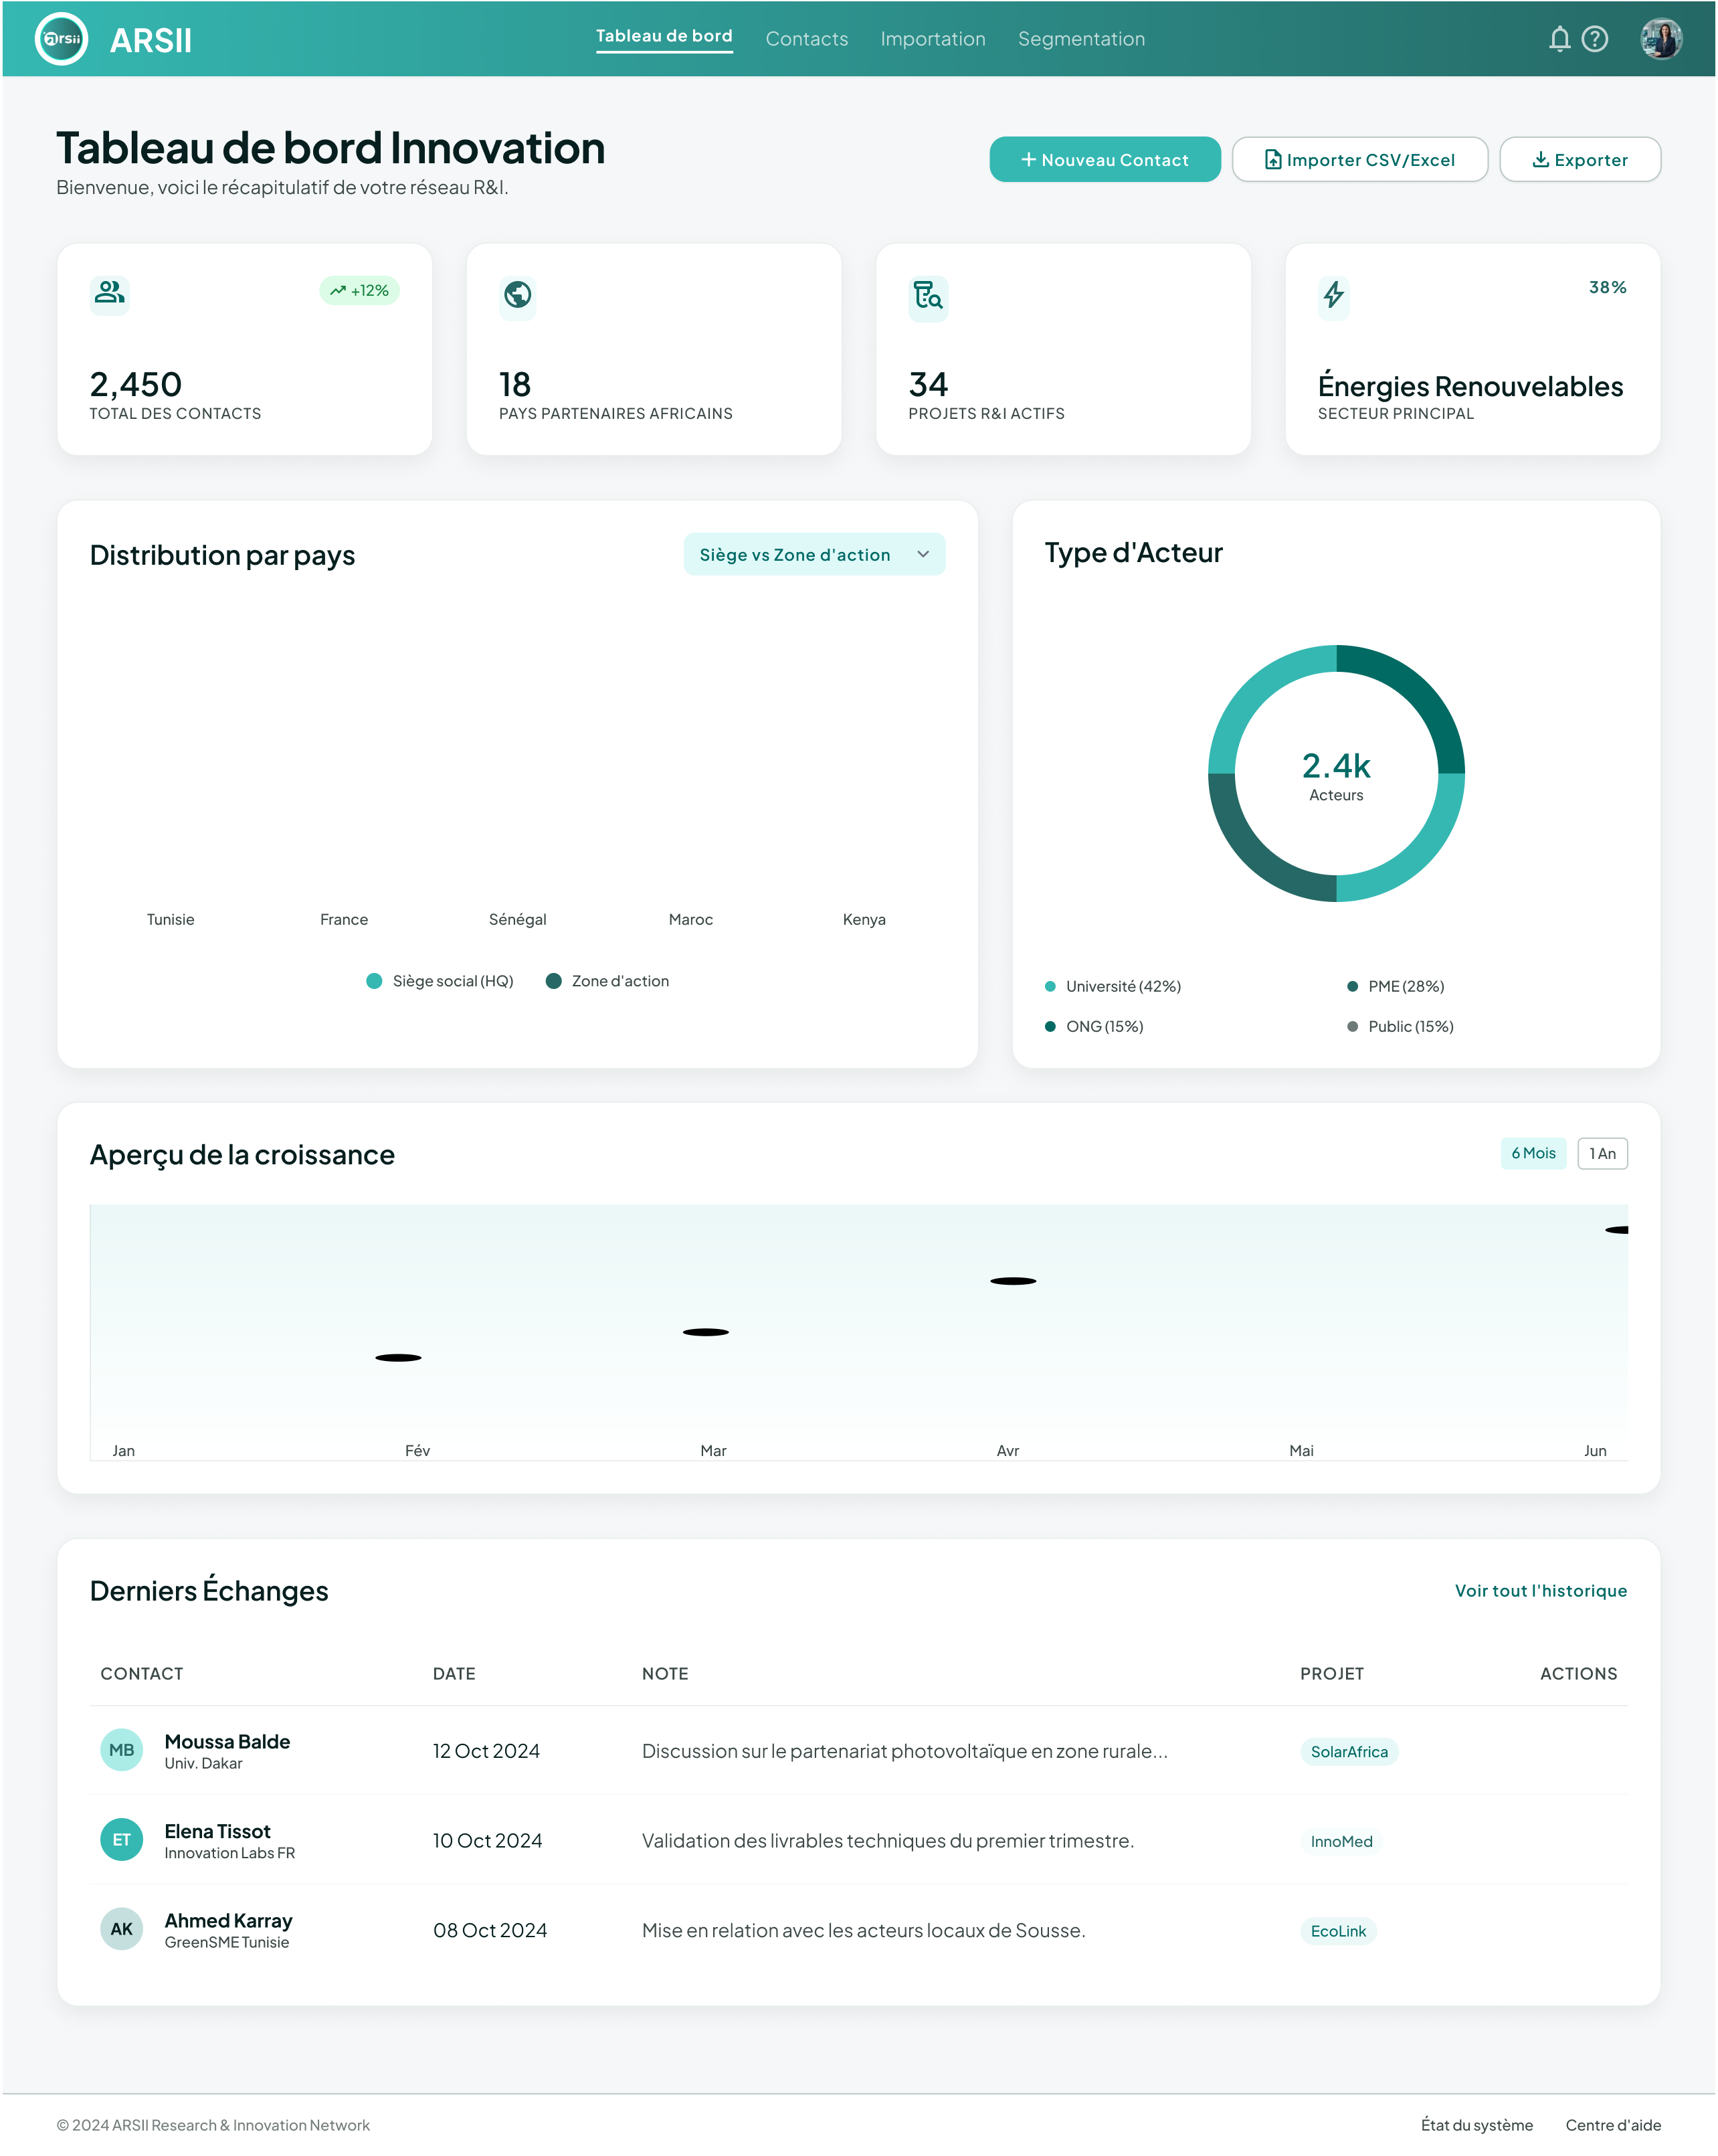
\includegraphics[width=0.9\textwidth]{images/maquette_dashboard.png}
\caption{Maquette : tableau de bord}
\label{fig:maquette-dashboard}
\end{figure}

Le choix du format de présentation vise une \textbf{prise en main rapide}, décliné par écran dans le tableau~\ref{tab:maquettes}.

\begin{table}[H]
\centering
\small
\begin{tabularx}{\textwidth}{|l|X|}
\hline
\textbf{Écran} & \textbf{Choix de conception} \\
\hline
Connexion & Écran minimal et centré \\
\hline
Liste des contacts & Tableau lisible, avec les actions principales accessibles \\
\hline
Fiche contact & Information regroupée de façon hiérarchisée \\
\hline
Tableau de bord & Indicateurs visuels de synthèse privilégiés \\
\hline
Assistant & Widget conversationnel accessible en permanence pour interroger la base \\
\hline
\end{tabularx}
\caption{Choix de conception pour les écrans principaux}
\label{tab:maquettes}
\end{table}

Ces choix ergonomiques répondent à l'exigence de convivialité des besoins non fonctionnels : l'interface se veut intuitive même pour un utilisateur non expérimenté.

Cette conception, de l'architecture au maquettage, fournit un cadre complet et cohérent pour la réalisation. Le chapitre suivant en détaille la mise en œuvre.
